\section{PROVABGS SED Modeling} \label{sec:provabgs}
% brief explanation of the PROVABGS SED modeling 
For each BGS EDR galaxy, we derive its $M_*$ and other properties,
$\overline{\rm SFR}$, $Z_{\rm MW}$, and $t_{\rm age, MW}$ from DESI
photometry and spectroscopy using the PROVABGS SED modeling
framework~\citep{hahn2022}.  
PROVABGS models galaxy SEDs using stellar population synthesis with
non-parametric star-formation history (SFH) with a starburst, a non-parametric
metallicity history (ZH) that varies with time, and a flexible dust
attenuation prescription.
The non-parameteric SFH and ZH prescriptions are derived from SFHs and ZHs of
simulated galaxies in the Illustris hydrodynamic
simulation~\citep{vogelsberger2014, genel2014, nelson2015} and provide compact 
and flexibly representations of SFHs and ZHs.
For the stellar population synthesis, PROVABGS uses the Flexible Stellar
Population Synthesis~\citep[FSPS;][]{conroy2009, conroy2010b} model with MIST
isochrones~\citep{paxton2011, paxton2013, paxton2015, choi2016, dotter2016},
\cite{chabrier2003} initial mass function (IMF), and a combination of
MILES~\citep{sanchez-blazquez2006} and BaSeL~\citep{lejeune1997, lejeune1998,
westera2002} spectral libraries.

Furthermore, PROVABGS provides a Bayesian inference framework for inferring
full posterior probability distributions of the SED model parameter:
$p(\theta\given {\bf X}^{\rm photo}, {\bf X}^{\rm spec})$, where ${\bf X}^{\rm
photo}$ represents the photometry and ${\bf X}^{\rm spec}$ represents the
spectroscopy. 
In total, $\theta$ has 13 parameters: $M_*$, 6 parameters specifying the SFH
($\beta_1, \beta_2, \beta_3, \beta_4, f_{\rm burst}, t_{\rm burst}$), 2
parameters specifying ZH ($\gamma_1, \gamma_2$), 3 parameters specifying
dust attenuation ($\tau_{\rm BC}, \tau_{\rm ISM}, n_{\rm dust}$), and a
nuisance parameter for the fiber aperture effect. 
Posteriors have distinct advantages over point estimates because they
accurately estimate uncertainties and degeneracies among galaxy properties.
Furthermore, as we later demonstrate, they are essential for principled
population inference: \eg~SMF.  

In practice, accurately estimating a 13 dimensional posterior requires a large
number ($\gtrsim$100,000) SED model evaluations, which would require
prohibitive computational resources. 
To address this challenge, PROVABGS samples the posterior using the
\cite{karamanis2020} ensemble slice Markov Chain Monte Carlo (MCMC) sampling
with the {\sc zeus} Python package\footnote{https://zeus-mcmc.readthedocs.io/}.
PROVABGS further accelerates the inference by using neural emulators for the
SED models. 
The emulators are accurate to subpercent level and $>100\times$ faster than the
original SED model based on FSPS~\citep{kwon2022}. 
With {\sc zeus} and neural emulation, deriving a posterior takes $\sim$5 min
per galaxy with PROVABGS.
Moreover, \cite{hahn2022} demonstrated PROVABGS can accurately infer $M_*$
overall the full expected $M_*$ range of BGS, using forward modeled synthetic
DESI observations. 

\begin{figure}
\begin{center}
    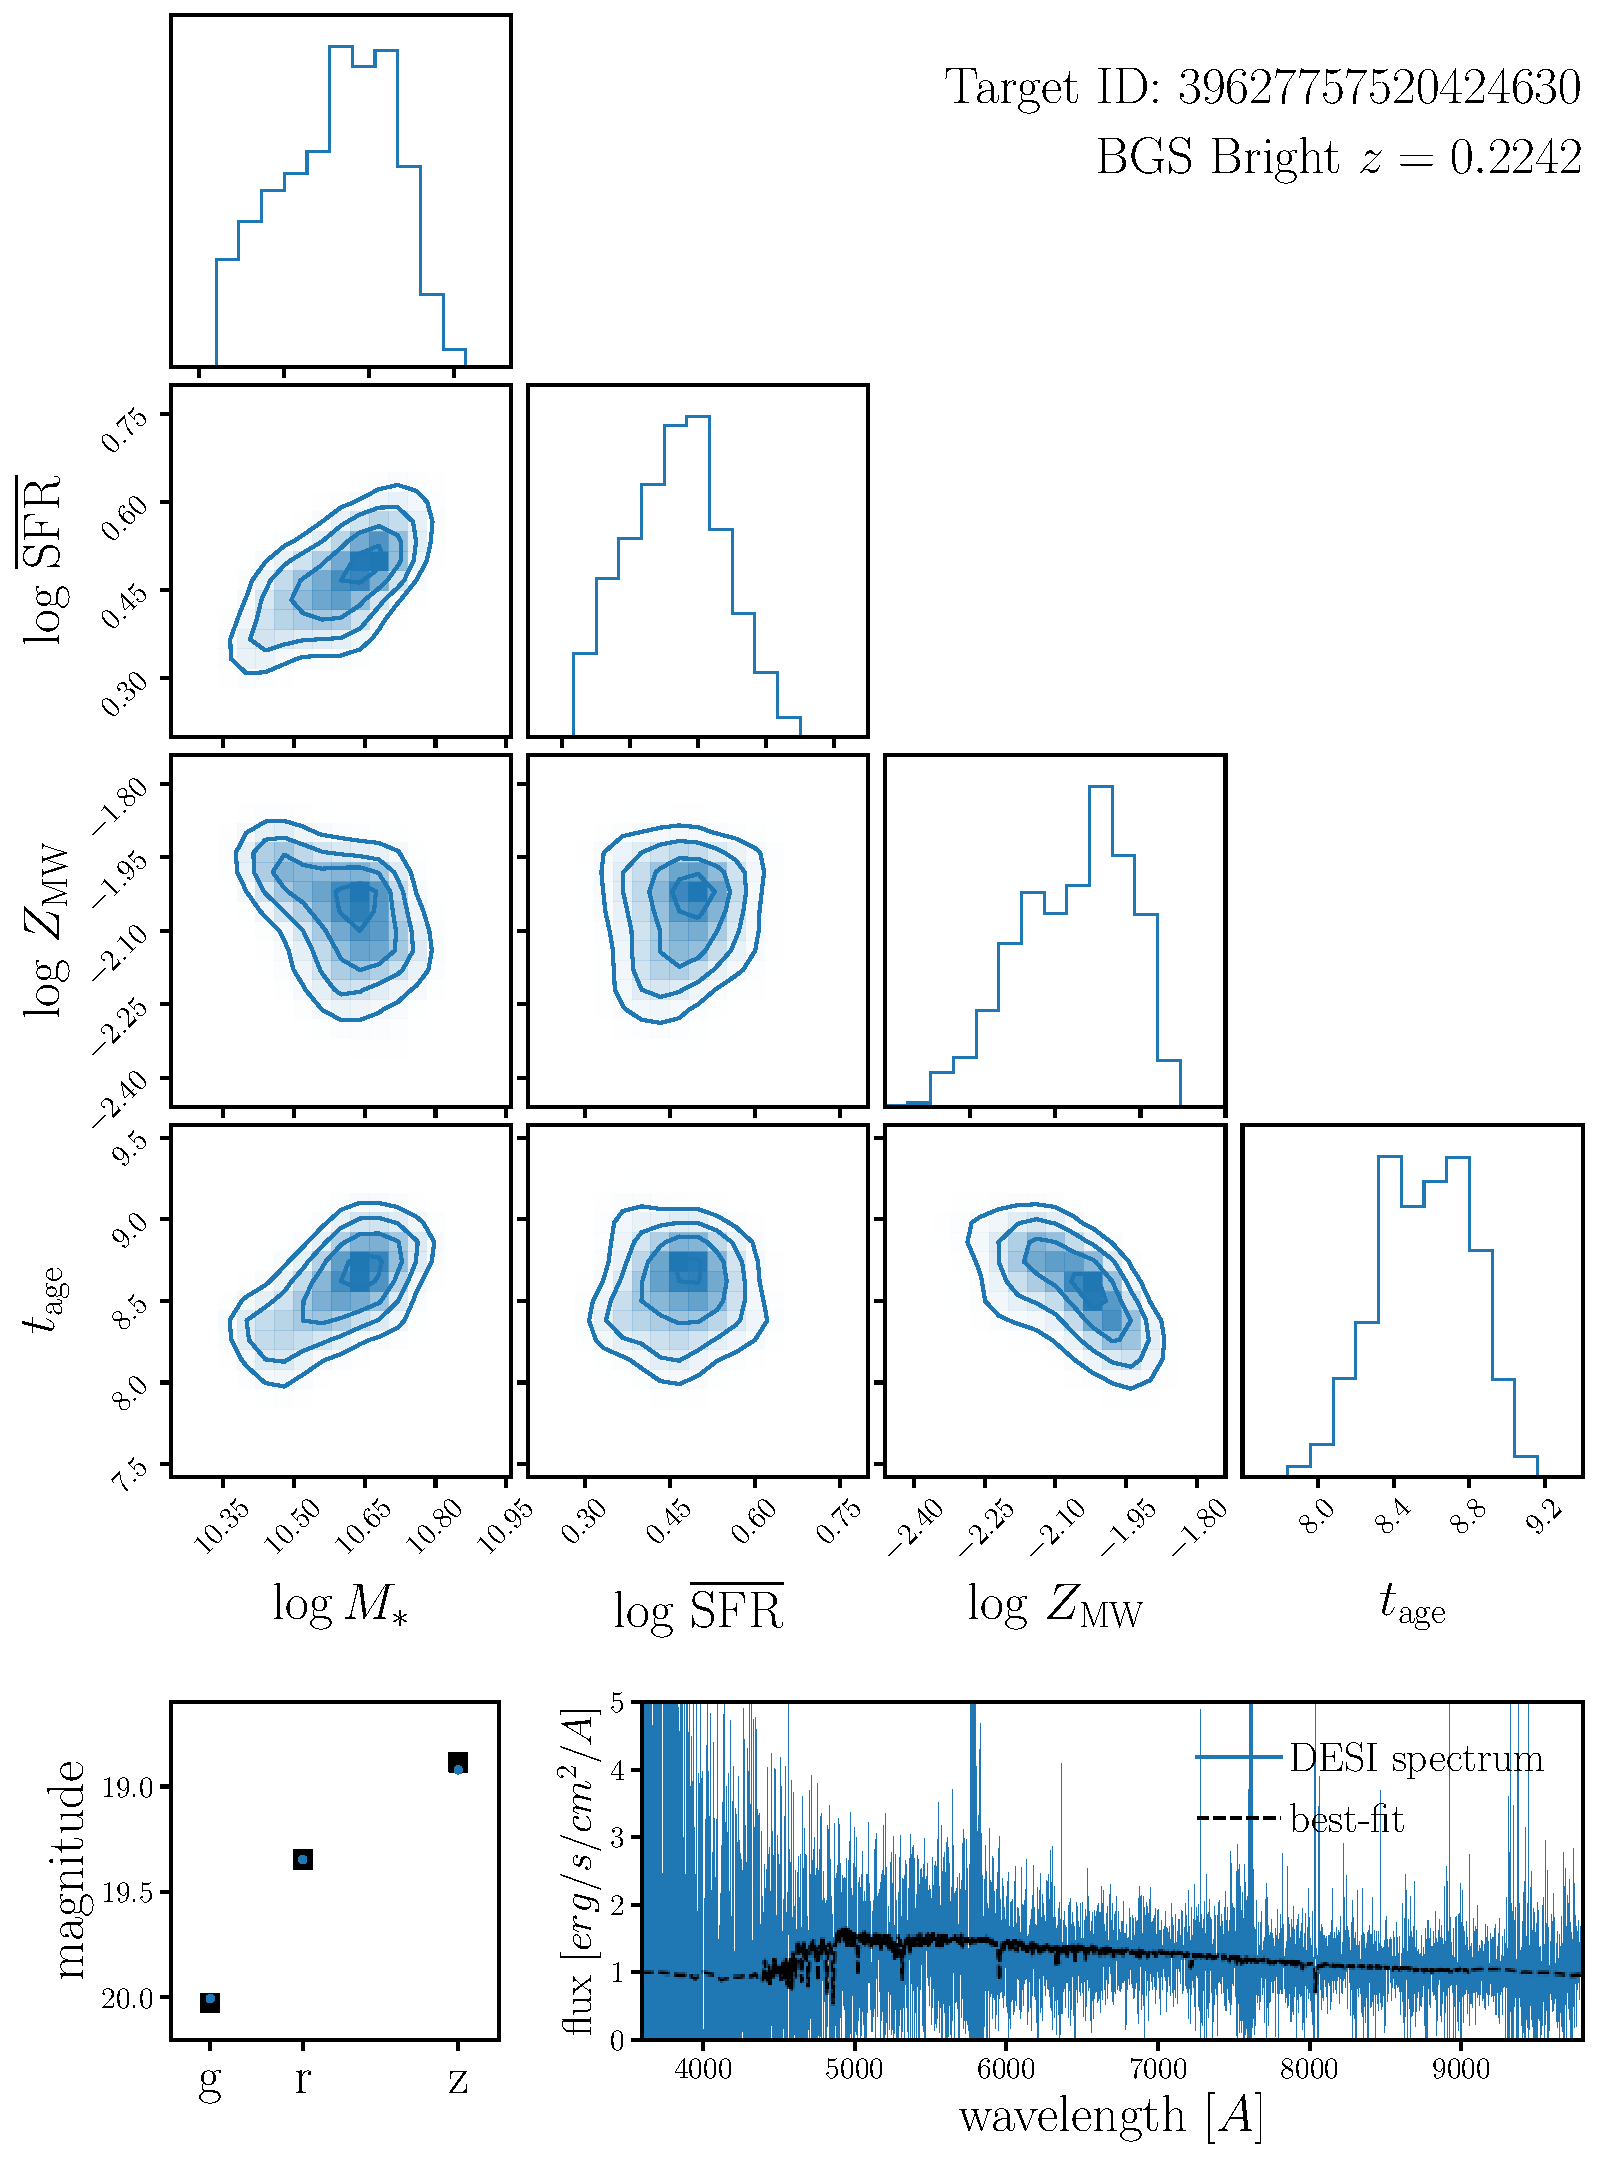
\includegraphics[width=0.6\textwidth]{figs/provabgs_posterior.pdf}
    \caption{
    }\label{fig:posterior}
\end{center}
\end{figure}


\begin{figure}
\begin{center}
    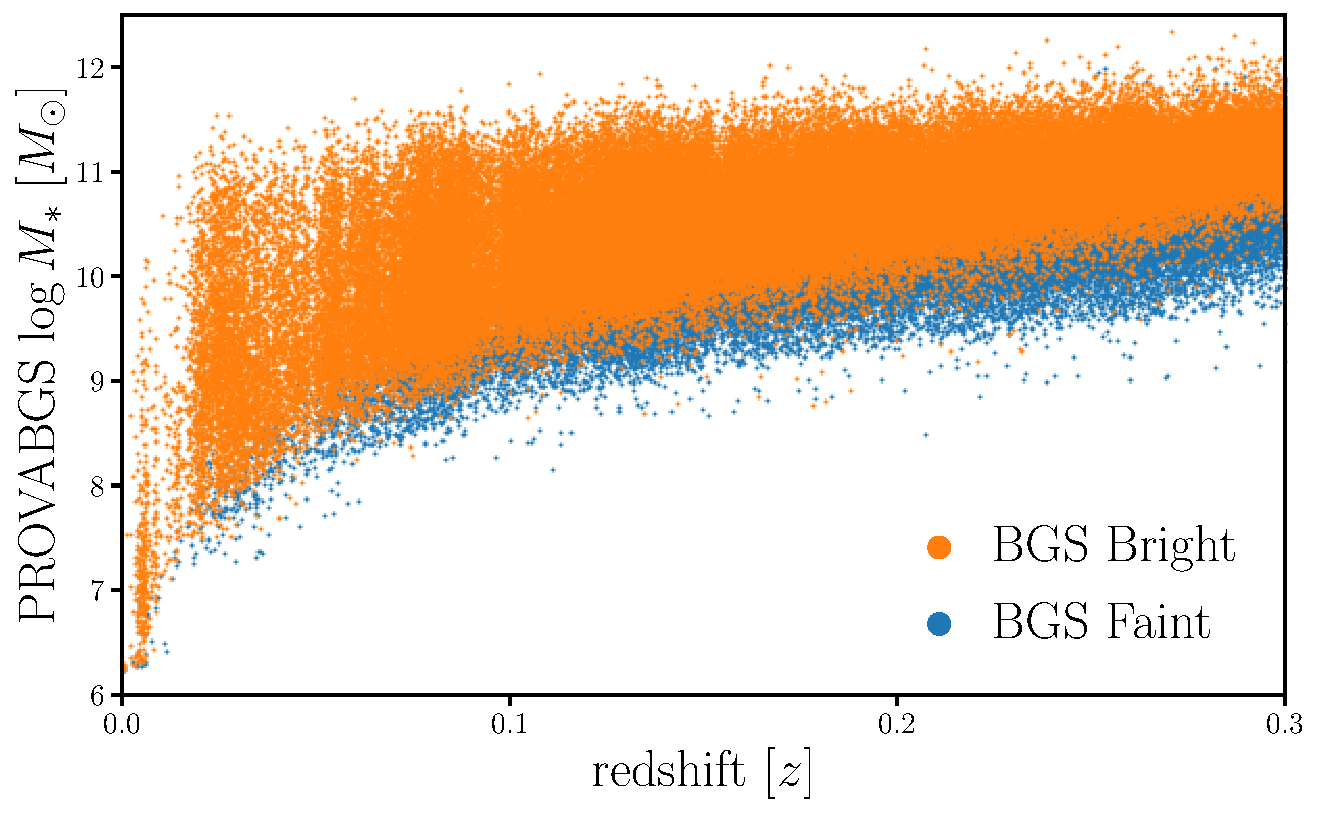
\includegraphics[width=0.6\textwidth]{figs/mstar_z.pdf}
    \caption{
    }\label{fig:mstar_z}
\end{center}
\end{figure}


In Figure~\ref{fig:posterior}, 

Figure~\ref{fig:mstar_z},
